
%
% $Id: slides.tex 4228 2006-06-21 21:55:12Z jjamor $
%
%
% Compilar a .pdf con LaTeX (pdflatex)
% Es necesario instalar Beamer (paquete latex-beamer en Debian)
%

%
% Gráficos:
% Los gráficos pueden suministrarse en PNG, JPG, TIF, PDF, MPS
% Los EPS deben convertirse a PDF (usar epstopdf)
%

\documentclass{beamer}
\usetheme{Warsaw}
\usebackgroundtemplate{
\includegraphics[width=\paperwidth]{format/libresoft-bg.png}}
\usepackage[english]{babel}
\usepackage[utf8]{inputenc}
\usepackage{graphics}
\usepackage{amssymb} % Simbolos matematicos
\usepackage{url}

%\definecolor{libresoftgreen}{RGB}{162,190,43}
%\definecolor{libresoftblue}{RGB}{0,98,143}

%\setbeamercolor{titlelike}{bg=libresoftgreen}

%% Metadatos del PDF.
\hypersetup{
  pdftitle={Libresoft},
  pdfauthor={Felipe Ortega},
  pdfcreator={GSyC/Libresoft},
  pdfproducer=PDFLaTeX,
  pdfsubject={Repositories with public data from FLOSS projects},
}
%%


\AtBeginSection[]
{
  \begin{frame}<presentation>
    \frametitle{Index}
    \tableofcontents[current]
  \end{frame}
}


\begin{document}

\title{Repositories with public data from FLOSS projects}
\subtitle{Master on Libre Software}
\institute{\\jfelipe@libresoft.es\\
GSyC/Libresoft}
\author{Felipe Ortega}
\date{\today}

\frame{
\maketitle
\begin{center}

\includegraphics[width=6cm]{format/gsyc-urjc}
\end{center}
}


% Si el titulo o el autor se quieren acortar para los pies de p�gina
% se pueden redefinir aqu�:
%\title{Titulo corto}
%\author{Autores abreviado}


%% LICENCIA DE REDISTRIBUCION DE LAS TRANSPAS
\frame{
~
\vspace{4cm}

\begin{flushright}
{\tiny
(cc) 2010 Felipe Ortega. \\
Some rights reserved. This document is distributed under the Creative \\
            Commons Attribution-ShareAlike 3.0 licence, available in \\
            http://creativecommons.org/licenses/by-sa/3.0/

%  Este documento (o uno muy similar) está disponible en \\
%  \url{http://gsyc.escet.urjc.es/~jjamor/}
}
\end{flushright}
}
%%

%%%%%%
%Transpas separadas por \begin{frame}
%%%%%%%%%%%%%%%%%%%%%%%%\end{frame}

\frame{
\frametitle{Table of contents}
\tableofcontents
}

\section{Introduction}

\begin{frame}
\frametitle{What is a meta-repository, anyway?}
\begin{itemize}
\item It is difficult to streamline the analysis of a long list of FLOSS projects.
\item Meta-repositories (or RoR, Repository-of-Repositories) simplify this problem.
\item They already serve metrics and metadata from FLOSS projects.
\item Help researchers and practitiones with metrics computation and compilation.
\end{itemize}
\end{frame}

\begin{frame}
\frametitle{Benefits from RoRs}
\begin{itemize}
\item Automated update of metrics and information gathered from FLOSS repositories.
\item Development of methodologies for analysis of FLOSS projects info.
\item Enabling analysis of large samples --> better results, broader coverage.
\item Reproducibility of research results.
\item Focus on the analysis, not data retrieval and cleaning.
\end{itemize}
\end{frame}

\begin{frame}
\frametitle{Available data}
\begin{itemize}
\item Metadata about projects
\item Source code
\item Issue Tracking information
\item Discussions
\item Documentation
\end{itemize}
\end{frame}

\begin{frame}
\frametitle{Common problems for data acquisition}
\begin{itemize}
\item Different platforms with different APIs.
\item Different formats to represent same info.
\item Performance issues.
\item Data loss.
\item Damage to project infrastructure.
\item Lack of expertise.
\end{itemize}
\end{frame}

\begin{frame}
\frametitle{Design conditions for RoRs}
\begin{itemize}
\item Accuracy.
\item Traceability.
\item Reproducibility
\item Completeness.
\item Respect to privacy.
\end{itemize}
\end{frame}

\begin{frame}
\frametitle{Two examples of RoRs}
\begin{itemize}
\item FLOSSmole.
\item FLOSSMetrics.
\end{itemize}
\end{frame}

\section{FLOSSmole}

\begin{frame}
\frametitle{FLOSSMole Factsheet}
\begin{itemize}
\item \url{http://flossmole.org/}
\item 350 GB data, period 2004 - present.
\item 500,000 different FLOSS projects.
\item Many different sources:
\begin{itemize}
 \item Forges: SourceForge, Rubyforge, Savannah, Github, Tigris, GoogleCode...
 \item Software lists: Freshmeat, SourceKibitzer, FSF Collections...
\end{itemize}
\item Different data export formarts:
\begin{itemize}
 \item Plain text (tab-delimited), downloadable SQL, live query tool (direct DB access).
\end{itemize}

\end{itemize}
\end{frame}

\begin{frame}
\frametitle{FLOSSMole factsheet}
\begin{itemize}
\item They also accept donations from individuals/research groups.
\item Discussion list for research community.
\begin{itemize}
 \item \url{http://sourceforge.net/mail/?group_id=119453}
\end{itemize}
\item Examples:
\begin{itemize}
 \item \url{http://flossmole.org/examples}
\end{itemize}

\end{itemize}
\end{frame}

\section{FLOSSMetrics}

\begin{frame}
\frametitle{FLOSSMetrics factsheet}
\begin{itemize}
\item \url{http://flossmetrics.org}
\item EU FP6 project funded by European Commission.
\item Fully operational since 2009.
\item Analysis of public data from FLOSS projects.
\item +2,800 projects analyzed:
\begin{itemize}
 \item +2,000 source code projects.
 \item +1,400 issue tracking systems.
 \item +600 mailing lists.
\end{itemize}
\end{itemize}
\end{frame}

\begin{frame}
\frametitle{FLOSSMetrics factsheet}
\begin{itemize}
\item Data retrieval: Blackbird.
\begin{itemize}
 \item \url{http://git.libresoft.es/blackbird}
\end{itemize}
\item Data analysis tools:
\begin{itemize}
 \item Libresoft tools: CVSAnalY, Mailing List Stats, Bicho.
 \item Community tools: CMetrics, CCCC, PyMetrics, PerlMetrics, SLOCCOunt.
\end{itemize}
\item Publishing web interface: Melquiades.
\begin{itemize}
 \item \url{http://melquiades.flossmetrics.org}
 \item Per project info: description, results, resources, charts, quality indicators (QualOSS), dumps.
\end{itemize}

\end{itemize}
\end{frame}

\section{Comparison between RoRs}

\begin{frame}
\frametitle{FLOSSMetrics factsheet}
\begin{itemize}
\item FLOSSMetrics == depth (source code, issue tracking...).
\item FLOSSMole == breadth (descriptive info, community, team size...).
\item Othe examples:
\begin{itemize}
 \item SRDA. The Sourceforge Research Data Archive.
 \item PROMISE Software Engineering Repository.
\end{itemize}

\end{itemize}
\end{frame}

\begin{frame}
\frametitle{FLOSSMetrics charts}
\begin{center}
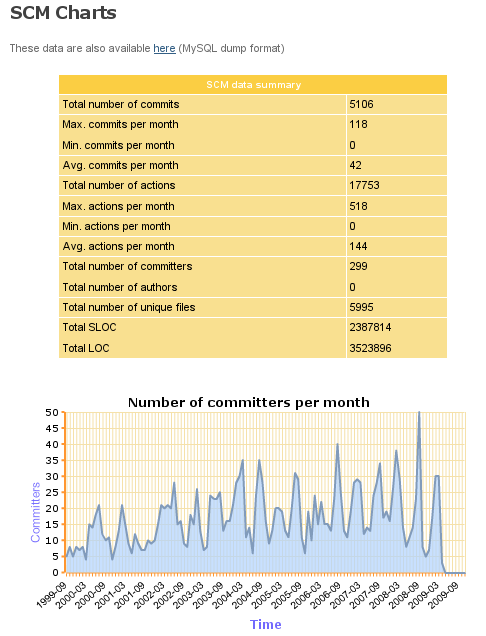
\includegraphics[width=0.45\textwidth]{figs/fm3-charts.png}
\end{center}
\end{frame}

\begin{frame}
\frametitle{FLOSSMetrics quality indicators (QualOSS)}
\begin{center}
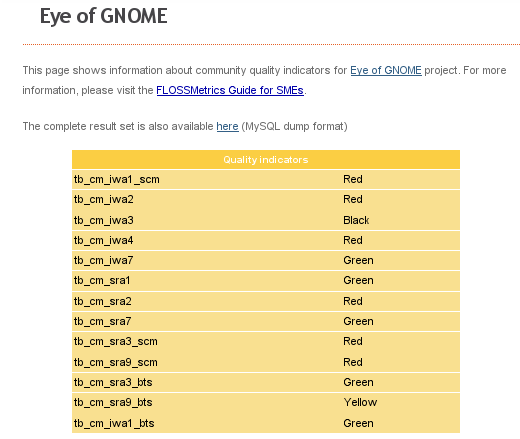
\includegraphics[width=0.65\textwidth]{figs/fm3-quality-indicators.png}
\end{center}
\end{frame}

\begin{frame}
\frametitle{FLOSSMetrics quality indicators (QualOSS)}
\begin{center}
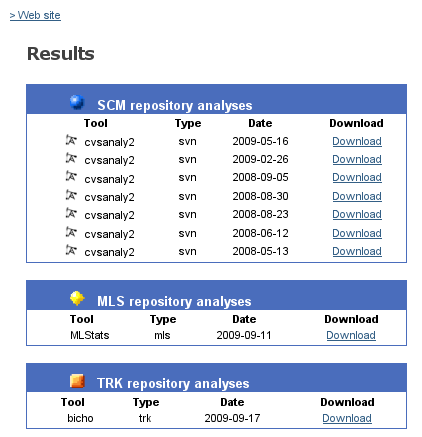
\includegraphics[width=0.5\textwidth]{figs/fm3-results.png}
\end{center}
\end{frame}

\begin{frame}
\frametitle{FLOSSMetrics quality indicators (QualOSS)}
\begin{center}
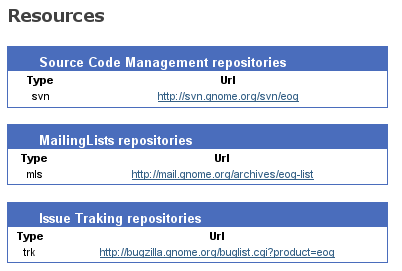
\includegraphics[width=0.6\textwidth]{figs/fm3-resources.png}
\end{center}
\end{frame}

\end{document}